% small.tex
\documentclass{beamer}
\usetheme{Boadilla}
\usepackage{graphicx}
\usepackage{wrapfig}
%algorithms and pseudo code
\usepackage{algorithm}
\usepackage[noend]{algpseudocode}
\usepackage{numprint}
\usepackage{subcaption}
\usepackage{media9}
\usepackage{bibentry}
\nobibliography*

\setbeamertemplate{bibliography item}[text]
\setbeamertemplate{author in head/foot}{\insertshortauthor}
\setbeamertemplate{navigation symbols}{}

\newcommand{\lenitem}[2][.6\linewidth]{\parbox[t]{#1}{\strut #2\strut}}
\newcommand{\outline}{
  \begin{frame}<beamer>
    \frametitle{Outline}
    \tableofcontents[currentsection]
  \end{frame}
}

\begin{document}

\title[Unstructured Mesh Workflows]
{
Dynamic Load Balancing of Massively Parallel Unstructured Meshes
}
\author{Gerrett Diamond, Cameron W. Smith, Mark S. Shephard}
%\email{diamog@rpi.edu}
%\author[smithc11@rpi.edu]{Cameron W. Smith\\
%  \smallskip
%  Committee:\\
%  Mark Shephard\\
%  Max Bloomfield, Christopher Carothers, Barbara Cutler, Onkar Sahni
%}

\institute[SCOREC]{
Scientific Computation Research Center \\
Rensselaer Polytechnic Institute
}

\date{November 13, 2017}

%----------- titlepage ----------------------------------------------%
\begin{frame}[plain]
  \titlepage
\end{frame}

%----------- outline ----------------------------------------------%
\begin{frame}
  \frametitle{Outline}
  \tableofcontents
\end{frame}

%----------------------------------------------------------------------%
%----------- Section --------------------------------------------------%
%----------------------------------------------------------------------%
\section{Partitioning and Load Balancing}
\begin{frame}
  \frametitle{Movtivation \& definitions}
  Many evolving distributed simulations have: \\
  \begin{itemize}
    \item Complex relational structures.
    \item Irregular forms of computational and communication costs.
    \item Evolving imbalance of work. %Define Imbalance
    \item Multiple levels of load.
  \end{itemize}
\end{frame}

\begin{frame}
  \frametitle{Common Methods for Partitioning}
  \begin{itemize}
  \item Multilevel Graph Methods %Discuss poor scaling
    \begin{itemize}
    \item ParMETIS
    \item Scotch
    \end{itemize}
  \item Geometric Methods %Require coordinates
    \begin{itemize}
    \item Recursive Coordinate Bisection (RCB)
    \item Recursive Inertial Bisection (RIB)
    \end{itemize}
  \item Diffusive Methods %Improve a partition efficiently
    \begin{itemize}
    \item ParMA
    \item EnGPar
    \end{itemize}
  \end{itemize}
\end{frame}

%Maybe one more slide to discuss in more detail why we need diffusive load balancing

\section{EnGPar - a graph based diffusive load balancer}

\begin{frame}
  \frametitle{What is EnGPar?}
  \begin{itemize}
  \item A diffusive load balancer to deal with multi-criteria partitioning.
  \item Utilizes a specialized graph structure to represent relation based data.
  \item Implemented to support efficient data parallel operations on GP-GPUs and vector units in many core processors.
  \end{itemize}
\end{frame}

\begin{frame}
  \frametitle{Software}
  EnGPar's source can be found at \url{https://github.com/SCOREC/EnGPar}.
  \begin{itemize}
  \item Written in C++ using MPI.
  \item Utilizes CMake for building.
  \item Depends on a SCOREC developed communication library, PCU.
  \item Future GPU work will use Kokkos.
  \end{itemize}
\end{frame}

\begin{frame}
  \frametitle{N-graph}
  %EnGPar utilizes an expanded multigraph structure called the N-graph.\\
  %THIS IS TOO MUCH TEXT PROBABLY...
  The N-graph has two modes of operation: traditional or hypergraph.\\
  \smallskip
  The N-graph is defined as the following:
  \begin{itemize}
  \item A set of vertices $V$ representing the atomic units of work.
  \item If using the traditional graph mode:
    \begin{itemize}
    \item $N$ sets of edges $E_0,...,E_{n-1}$ for each type of relation.
    \item Each edge connects two vertices $u,v \in V$.
    \end{itemize}
  \item If using the hypergraph mode:
    \begin{itemize}
    \item $N$ sets of hyperedges $H_0,...,H_{n-1}$ for each type of relation.
    \item $N$ sets of pins $P_0,...,P_{n-1}$ corresponding to each set of hyperedges.
    \item Each pin in $P_i$ connects a vertex, $v \in V$, to a hyperedge $h \in H_i$.
    \end{itemize}
  \end{itemize}
\end{frame}

\begin{frame}
  \frametitle{Mapping structures to the N-graph}
  %Before using EnGPar a simulation must first map its data to the N-graph
  To map to the N-graph simulations must:
  \begin{itemize}
  \item Define units of work as the vertices.
  \item Decide on the method of edges to use.
  \item Define the relations between the work as (hyper)edges.
  \end{itemize}
  
  %Figure showing the conversion from mesh to N-graph
  \begin{figure}
    \centering
    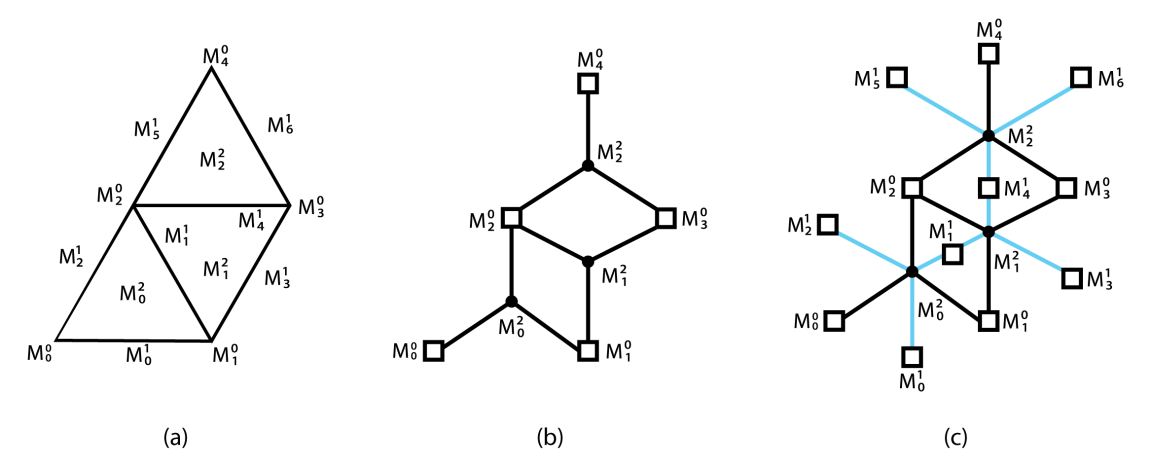
\includegraphics[width=.7\textwidth]{figures/exampleMesh2Graph.png}
  \end{figure}
\end{frame}

\begin{frame}
  \frametitle{Diffusive Partitioning}
  \begin{algorithm}[H]
    \caption{Diffusive Load Balancing Framework}
    \label{alg:engpar}
    \small
    \begin{algorithmic}[1]
      \Procedure{Balance}{$ngraph$,$dimensions$}
      \ForAll{$d \in dimensions$}
      \While{imbalance of $d >$ tolerance}
      \Call{RunStep}{$ngraph$,$d$}
      \If{Balancing Stagnates}
      \State break
      \EndIf
      \EndWhile
      \EndFor
      \EndProcedure

      \Procedure{RunStep}{$ngraph$,$d$}
      \State $sides = makeSides(ngraph)$
      \State $weights = makeWeights(ngraph,sides,d)$
      \State $targets = makeTargets(ngraph,sides,weights)$
      \State $queue = makeIterationQueue(ngraph)$
      \State $plan = select(ngraph,targets,queue)$
      \State $trim(ngraph,plan)$
      \State $ngraph.migrate(plan)$
      \EndProcedure
    \end{algorithmic}
  \end{algorithm}
\end{frame}

%More slides to describe each step with some detail
\begin{frame}
  \frametitle{Neighbor Initialization}
  \begin{itemize}
  \item Sides
    \begin{itemize}
    \item Each part determines which parts are its neighbors.
    \item Determines a measurement of the length of the part boundary.
    \end{itemize}
  \item Weights
    \begin{itemize}
    \item Each part computes its weight of the current target dimension.
    \item This weight is shared with all of the parts neighbors(sides).
    \end{itemize}
  \item Targets
    \begin{itemize}
    \item Each part determines which part they will send weight to.
    \item Weight to send from part $i$ to part $j$ is $(w_i-w_j)*\dfrac{\text{size}(s_{ij})}{\text{size}(s)}$
    \end{itemize}
  \end{itemize}
\end{frame}

\begin{frame}
  \frametitle{Building the Migration Plan}
  \begin{itemize}
  \item Selection
    \begin{itemize}
    \item All (hyper)edges that cross a part boundary are iterated.
    \item The vertices on part that are bounded by the (hyper)edge form a cavity.
    \item The cavity is chosen for migration if the (hyper)edge is on the boundary of a targeted part.
    \end{itemize}
  \item Trim %This may be cut for time/understanding sake
    \begin{itemize}
    \item In the case of multiple criteria, the migration plan created through selection may be reduced.
    \item This reduction ensures that the weight being sent will not increase the previously balanced criteria.
    \end{itemize}
  \end{itemize}
\end{frame}


\begin{frame}
  \frametitle{Iteration Queue}
  %the edges on the boundary are ordered/not vertices
  In order to make well shaped parts, the order that vertices are selected matters. \\
  \bigskip
  To minimize part boundaries, the graph vertices on the part boundary are ordered based on their distance from the center of the part. \\
  \bigskip
  This results in more rounded parts and less surface area. 
  %This can be described much better. Maybe with a very high level algorithm.
\end{frame}


\section{Comparison to ParMA}

\begin{frame}
  \frametitle{Experiments}
  %Describe the mesh, system run on, initial partition etc.
\end{frame}

%More slides to go over the results in the paper

\begin{frame}
  \frametitle{Future Work}
  Expanding the capabilities of EnGPar:
  \begin{itemize}
    \item Improve partitioning structures at very high part count.
  \item Supporting the diffusive algorithms on GPUs
  \end{itemize}
  Applying EnGPar to other applications:
  \begin{itemize}
  \item CODES - a discrete event simulation for communication on supercomputer networks.
  \item FUN3D - a computational fluid dynamic simulation...
  \item PHASTA - I have no idea...
  \end{itemize}
\end{frame}

\begin{frame}
  \frametitle{Citations}
\end{frame}
  
\end{document}
